%!TEX root = ../thesis.tex

\section{実験概要}
本章では, 前章の実験で使用した教師データの何に問題があるかの調査を行う. 具体的には, 5章で最も成功率の高かった実験(以後, 実験1と呼ぶ)で使用した教師データと, 前章の実験(以後, 実験2と呼ぶ)で使用した教師データを入れ替えて学習を行う. これにより, 目標角速度とカメラ画像のどちらに問題があるか判明するのではないかと考える. 

\section{実験装置}
原因の調査を行うために, シミュレータを用いた実験を行う. 実験環境, 実験装置は前章と同様のシミュレータ環境を用いる. 

\section{実験方法}
学習器の訓練条件, 学習したモデルを用いたテストなどの条件は前章と同様とする. 実験1の目標角速度と実験2のカメラ画像の組み合わせを実験3, 実験1のカメラ画像と実験2の目標角速度の組み合わせを実験4とする

\subsection{実験結果と考察}
実験結果を\ref{tb:inves}に示す. 実験3の成功回数は

\begin{table}[h]
  \centering
  \caption{Number of successes in the experiments of simulator}
  \begin{tabular}{|c|c|} \hline
      Experiments & Number of successes \\ \hline
      Exp. 1 & 0/10 \\ \hline
      Exp. 2 & 9/10 \\ \hline
    \end{tabular}
  \label{tb:inves}
\end{table}

% 前章で最も成功率の高かった際の教師データを実験1, 本章の教師データを実験2として比較を行う. これにより, 目標角速度とカメラ画像に問題があるかを調査する. \figref{Fig:ratio}に目標角速度の割合を比較したグラフを示す. 

% \begin{figure}[h]
%   \centering
%   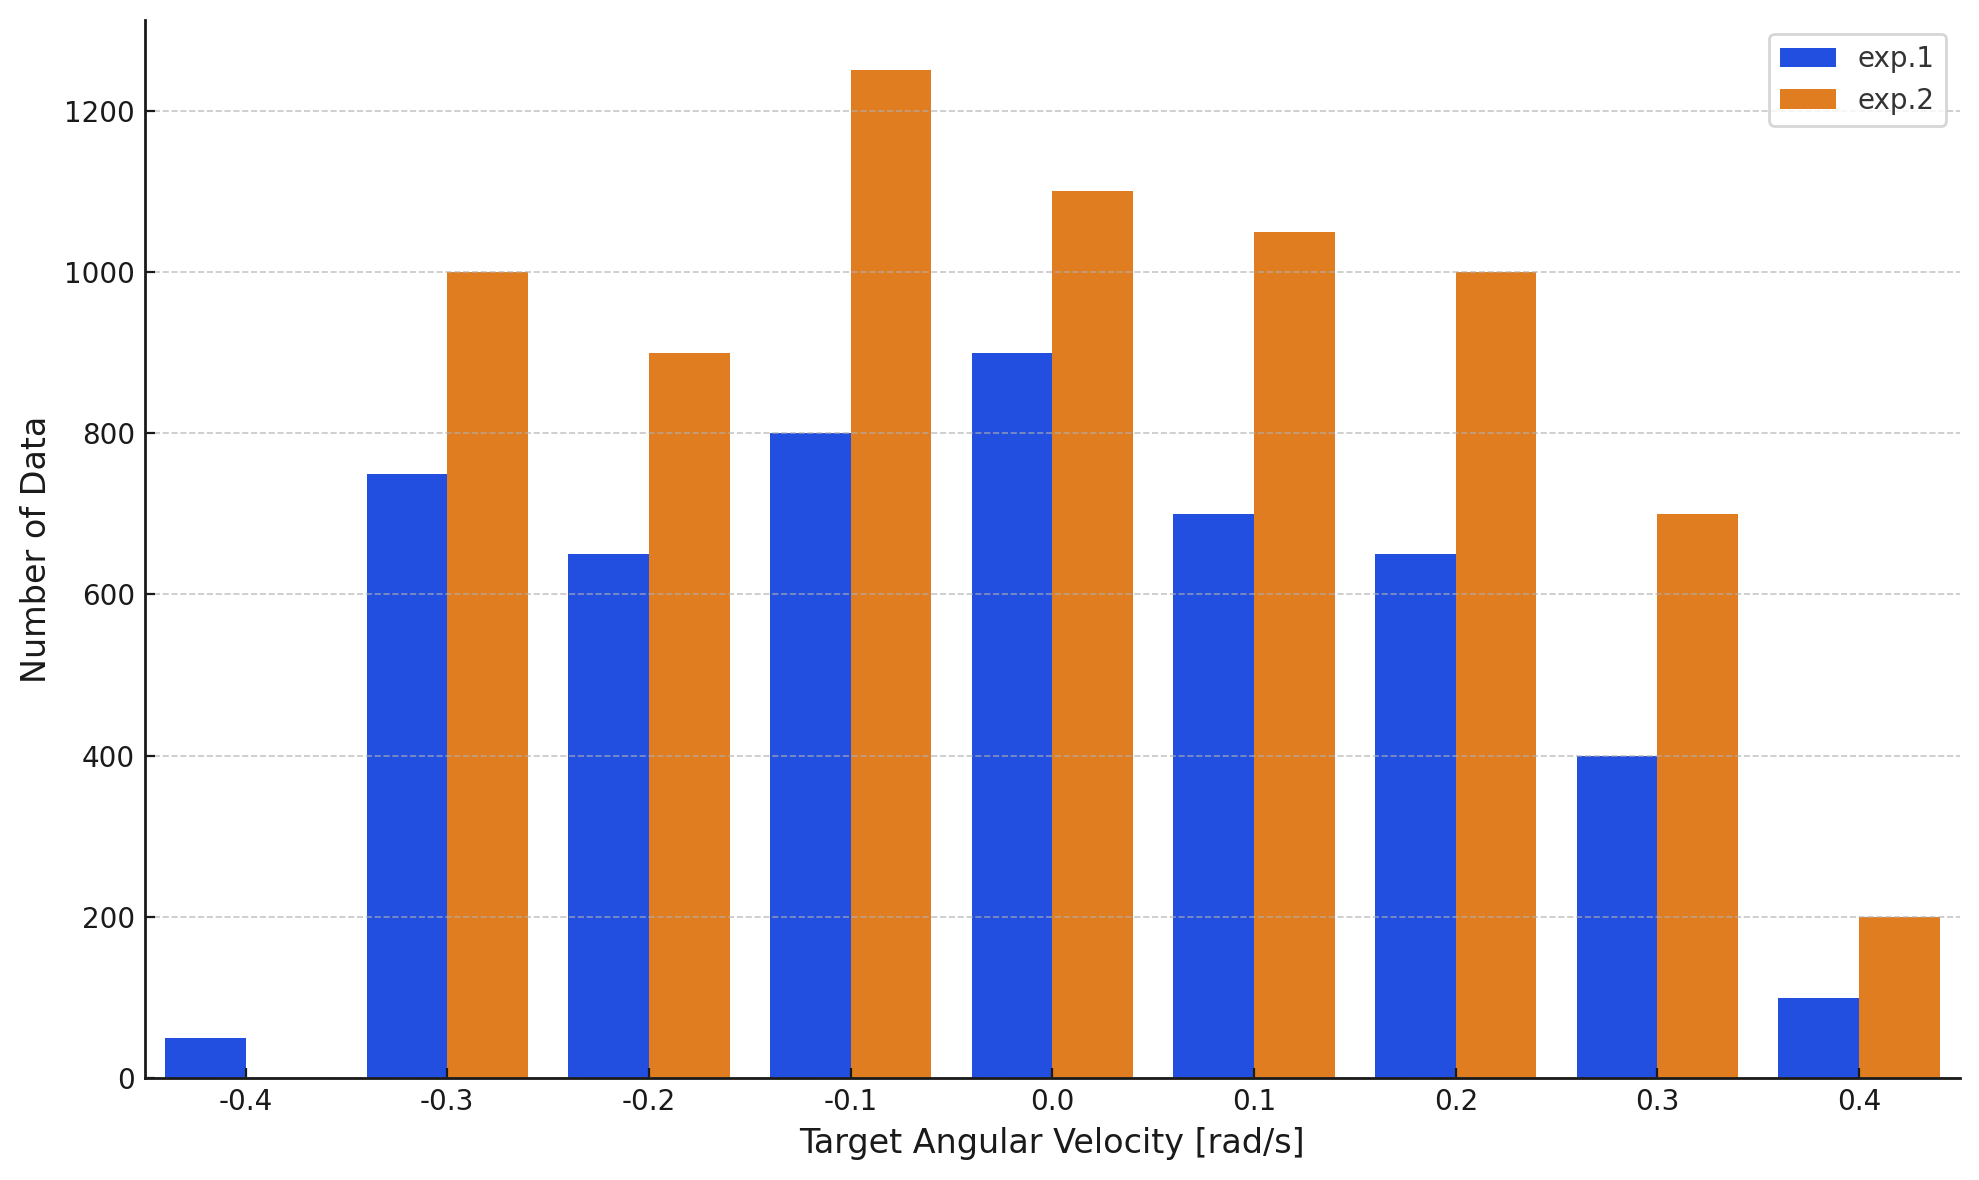
\includegraphics[keepaspectratio, scale=0.5]{images/output.png}
%   \caption{Comparison of target angular velocity ratios}
%   \label{Fig:ratio}
% \end{figure}

% 実験1と実験2の教師データを入れ替えて実験を行った. まず, 実験1のカメラ画像と実験2の目標角速度の組み合わせで学習を行った.